\chapter{DEFINICIÓN DEL PROBLEMA}
\label{chapter:problem}
\hyphenation{BeamCal}
\section{The BeamCal Instrumentation }

Por canal los componentes the Bean V2 son 
\begin{itemize}
\item Un amplificador sensible a la carga o CSA con pulsador de carga.
\item Un filtro de capacitores conmutados totalmente diferencial con supresión de filtro de baja frecuencia.
\item Un conversor análogo digital (ADC)de 10-bit tipo SAR
\item Una Memoria digital
\end{itemize}

\subsection{Requerimientos de diseño}
\begin{itemize}
\item Máxima carga por pixel: 36.9pC en SDT y 50 veces más chicos en DCal.
\item Considerando 10 bits de resolución, $1LSB = 225k$ electrones en la entrada (SDT) y $1LSB = 4.5k$ electrones en la entrada para el modo DCal.
\item Con solo $308ns$ para procesar señales el ruido serie es mas importante en el proceso por lo que $N_s= \int(W'(t))^2dt$ es decir, depende de la derivada de $W(t)$. Por lo tanto $W'(t)$ debe ser muy alta para definir la forma de pulso en un corto tiempo.
\item Cambien es necesario usar algún modo de restauración de baseline. Esto dado a que el \textit{front-end} es variante en el tiempo.
\item El $N_s$ mínimo corresponde a una forma de triangulo isósceles en $W(t)$ que minimiza la pendiente.
\end{itemize}
\subsection{Diseño del filtro a nivel de sistema}
La función implementada por el filtro es de la forma
\begin{equation}
F(z)= \sum_{0}^{N-1} a_{N-j}*z^{-j}
\end{equation}

Esta función es implementada con el filtro de la figura. La operación del filtro se basa en dos etapas: la primera etapa consiste en una etapa de muestreo o fase $\phi_1$ en la cual el voltaje de entrada carga al capacitor $C_s$. Durante la segunda etapa o etapa $\phi_2$ el corto circuito de la entrada fuerza a $C_s$ a pasar su carga a $C_f$. Al fin de la etapa $\phi_2$ la salida del filtro es igual al valor del ciclo anterior más $C_s V_i/C_f$.\\
Esta versión del filtro cuenta ademas con una version temprana de $\phi_1$ y es usada para la fase de muestreo con la intensión de implementar una técnica denominada \textit{bottom-plate sampling}.
El valor de $C_s$ es configurable digitalmente. En la figura XX se puede aprecia como esta implementado el condensador $C_s$, de este modo, según las señales \verb+CS_Bx+ se puede elegir la cantidad de condensadores en paralelo con la cual se quiere operar, cambiando de este modo la ganancia del filtro.\\
El filtro posee en la entrada multiplexores que permiten invertir el signo de la señal de entrada. Esto permite implementar una técnica denominada  CDS. La señal que controla este multiplexor es denominada \verb+sgn+.
El voltaje de modo común de salida del filtro es fijado automáticamente por un circuito de realimentación (CMFB), el cual necesita de una referencia externa. Por otro lado, el voltaje de modo común de la entrada es fijado por la referencia externa \verb+Vicm+.\\
Los multiplexores de la salida del OTA permiten que la señal evada el filtro, reflejando en la salida del filtro, las señales de su entrada. La señal que controla estos, multiplexores es denominada \verb+out\_s+.

\subsection{Prototipo}

La versión implementada en el integrado a probar es realmente una versión de prototipo de the Bean v2. Esta versión de prototipo incluye
\begin{itemize}
\item una versión simple de lectura de canal: Incluye 2 CSA, uno de los cuales presenta un cortocircuito entre su salida y su entrada para generar el \textit{baseline}.
\item un circuito de precarga.
\item el filtro SC diseñado.
\item buffers de salida.
\item una version aislada del filtro el cual cuenta con sus entradas conectadas directamente a pines del integrado para propósitos de caracterización del filtro.

\end{itemize}

Las señales más importantes se encuentran respectivamente buffereadas para poder se leidas con instrumentos de medición. 
\section{Diseño del circuito}
\subsection{Especificaciones generales}
\begin{table}
\begin{tabular}{|c|c|}
\hline 
Modos & SDT, DCal \\ 
\hline 
Capacitancia de entrada & 40pF \\ 
\hline 
Carga de entrada & 36.9pC(SDT), 738fC(DCal) \\ 
\hline 
Rango de salida & 1V o cercano \\ 
\hline 
Nolinealidad & <1\% (Medido como la máxima desviación del linear)\\ 
\hline 
Tiempo de establecimiento & <154ns \\ 
\hline 
\end{tabular} 
\caption{Especificaciones generales para el circuito que implementa el CSA}
\end{table}

La ecuación generica de un CSA es
\begin{equation}
v_o=\frac{Q_{in}}{C_F}\cdot (\frac{A_{ol}\beta}{1+A_{ol}\beta})=\frac{Q_{in}}{C_F}\gamma_{ol}
\end{equation}

En donde el valor de beta esta dado por
\begin{equation}
\beta=\frac{C_F}{C_F+ C_{(D+W)}}
\end{equation}

En esta ecuación podemos apreciar que para el caso en que $A_{ol}= \infty$, $v_o=\frac{Q_{in}}{C_F}$.
Por otro lado, debido a que $A_{ol}$ cambia dependiendo del rango de entrada, entonces el valor de $\gamma_{ol}$ introduce no linealidades mayores si $C_F$ es pequeño, como es en el caso del modo DCal.

Con todo lo anterior mencionado se deduce que valores adecuados para las capacitancias son  $C_F=45pF$ para el modo SDT y $C_F=0.9pF$ para el modo DCal. Con esto se obtiene un rango de 0.82V a la salida y una buena linealidad.

\section{Camino de la señal. obs: basado en the bean}

El CSA esta diseñado con un cascodo plegado( buena ganancia ancho de banda y 1.8V). El CSA posee dos condensadores para implementar la red de realimentación. La configuración de estos es ajustable por medio de señales digitales, lo que permite configurar la ganancia. Para un dispositivo con implementado en nmos en la entrada el baseline es ajustado a $V_T$ o 0.5V.\\
Para aprovechar mejor el rango de excursión de la salida del CSA, se conectará un circuito interno de precarga para inyectar una cantidad conocida de carga antes de cada ciclo. Esto con el fin de mover el baseline a un valor cercano a 0.4V.\\
El \textit{front-end} cuenta con un filtro después del CSA, el cual puede ser evitado dependiendo del modo de operación, lo cual es seleccionable por medio de una señal digital.\\
El filtro implementado es un integrador sin perdidas para tener una pendiente de una función triangular.
\begin{itemize}
\item El filtro se implementa por medio de un integrador diferencial de capacitores conmutados (SC).
\item Debido a la naturaleza de muestreo de los SC ocurre aliasis de componentes de alta frecuencia (incluso ruido) por lo que aparecen en la banda base.
\item Idealmente la frecuencia de corte (o ancho de banda) del CSA deben servir como filtro antialiasis.
\end{itemize}
La frecuencia óptima para los SC es $51.95MHz$ esto se debe a que se consideran 16 muestras por colisión considerando una frecuencia de $3.2MHz$ tenemos en total $f=51.95MHz=3.2MHz*16$. 16 ciclos representan un buen \textit{trade-off} entre complejidad y desempeño.\\
The bean debe procesar  entradas a una taza de $3.247MHz$ con un cloc interno de 16 veces más rápido. De este modo el periodo de $308ns$ entre pulsos constituye 1 ciclo los $16$ \textit{clock} en cada siclo son un sub-ciclo y periodos de muestreo de los capacitores conmutados.\\
Cuando se selecciona la opción de evitar el filtro, la pendiente negativa del filtro esta relacionado con la pendiente de la respuesta en el tiempo del CSA. Por otro lado cuando el filtro es incluido, la pendiente negativa es formada por el filtro del SC. El filtro es mejor para el ruido pero consume más corriente.\\
La pendiente negativa es implementada por medio de un método denominado \textit{correlated doulbe sampling} (CDS).\\
Es necesario al menos un ADC de $3.24MHz$ a la salida del sistema.
\section{Presupuesto de ruido y potencia}
Alcanzar los 2.19 mW es difícil por que el CSA consume la mitad aproximadamente. Sin embargo es posible implementar una metodología para reducir los consumos, la cual consiste en apagar o reducir el consumo de corriente en los tiempos inactivos o periodos de silencio (los cuales representan aproximadamente el 99.5\% del tiempo total). La potencia finalmente no es un problema.
El ruido total a la entrada debe ser $65k$ electrones en el modo SDT. y $1.3k$ en modo DCal.
\section{Timing. OBS basado en the bean}
El camino comienza con el CSA, conectando al detector  por condenzadores de acoplamiento externo.\\
Existe un pulsador interno con el fin de calibrar las señales conocidas.\\
El pulsador dobla como un circuito de precarga. Mueve el \textit{baseline} para tomar mayor ventaja de la región lineal del CSA.\\
Después del CSA viene un filtro integrador de capacitores conmutados, capaz de producir tanto la pendiente triangular negativa como la pendiente positiva (CDS).

Posteriormente a continuación del SC viene un ADC el cual puede elegir si lee desde el CSA o desde el filtro. La salida del ADC es leída en los tiempos de silencio u son guardados en memorias digitales.\\
En los cascodos plegados el \textit{baseline} es aproximadamente establecido por el voltaje de umbral:$V_{DD}-\vert V_{TH}\vert$ para dispositivos con Pmos y $V_{th}$ para dispositivos con Nmos.\\
Es necesario un circuito de pre-carga para mover el \textit{baseline} y aprovechar mejor la región lineal del CSA.\\
La etapa de realimentación se implementa con dos capacitores $C_{op}$ y $C_{cal}$ y dos switches que permiten tanto resetear los condensadores como elegir el modo de operación.\\
Durante la etapa de aplificación la señal de reset permanece abierta. Cuando se relaiza un full reset, los switches de reset son controlados por $R_{stf}$. Pasados los cuatros ciclos de full reset la carga guardada en los capacitores de realimentación es despreciable y el la señal de control de $R_{stf}$ es desabilitado.
\section{Pre charger}
La función principal de este circuito es inyectar carga conocida al CSA para ajustes en el baseline. El condensador $C_{pc}$ es de $C_pc=0.5pF$ el cual es usado para el modo Dcal. Existe la opción de conectar un condensador 50 veces mas grande desde fuera del chip para precarga en el modo SDT.
El circuito de precarga funciona con dos clock desfasados no solapados $\phi_1$ y $\phi_2$. Durante $\phi_1$ el lado izquierdo de $C_{pc}$ es conectado a un voltaje de referencia externo $V_{DD\_ref}$. Durante $\phi_2$ el lado izquierdo de $C_{pc}$ es conectado a GND. En cada transición de $\phi_1$ a $\phi_2$ el capacitor inyecta $Q_{pc}=C_{pc} V_{DD\_reff}$ en la entrada del CSA. Esto produce una diferencia de voltaje a la salida del CSA de $\frac{-C_{pc}V_{DD\_reff}}{C_F}$.
En donde $C_F$ es $C_{cal}$ en el modo Dcal. y $C_{cal}+C_{op}$ en el modo SDT.\\

La inyección de carga es realizada justo despues de que el CSA es habilitado (salir del estado de reset). Reduciendo de este modo el voltaje de salida a la salida.\\

Desde luego ocurre una transición opuesta cuando operamos desde $\phi_1$ a $\phi_2$ sin embargo, esta rutina ocurre en el estado de reset por lo que el baseline no se ve afectado por esta transición.


The work described in this thesis is a contribution to the design and implementation of the front-end circuit for one of the detector systems of the International Linear Collider (ILC). The project is endorsed by the ILC Forward Calorimetry Collaboration (FCAL), a worldwide detector research and development collaboration, and party sponsored by CONICYT through the FONDECYT Program.

Planned to be operating in the mid 2020’s, the ILC will be the largest linear particle collider ever built. Consisting of two linear accelerators that will stretch approximately 32 kilometers in length, the ILC will smash electrons and positrons together at nearly the speed of light. The intended beam collision energy is 500 billion-electron-volts (GeV) for the first stage, with the possibility for a later upgrade to 1 TeV. 
 
Located at the ILC detector forward region, the BeamCal is a highly segmented \mbox{($>$ 90000 channels)} calorimeter that will serve four main purposes: improve the hermeticity of the ILC detector for low polar angles, reduce the backscattering from pairs into the inner ILC detector part, protect the final magnet of the beam delivery system, and assist the beam diagnostics. The BeamCal specifications for radiation tolerance, noise, signal charge, pulse rate and occupancy pose unique challenges for the instrumentation system. Although initially planned  for the ILC, the BeamCal calorimeter could also be used in the Compact Linear Collider (CLIC), the alternative particle accelerator in race to follow the LHC.

The FONDECYT project \#11110165: Application of Advanced CMOS Techniques in Pulse Processors for Particle Physics Experiments deals with the design and implementation of a mixed-signal application-specific integrated circuit (ASIC) to address the BeamCal instrumentation needs. The IC, called the Bean, will be designed for a standard 180-nm CMOS process and will be based on a 3-channel prototype developed in a previous work \citep{abusleme101}. Each independent channel will include: a charge-sensing amplifier with a pre-charging pulser; a fully differential switched-capacitor (SC) filter with a low-frequency noise suppression feature; a 10-bit, fully-differential, successive approximation register (SAR) charge redistribution analog-to-digital converter (ADC); and a digital storage array. Additionally, the IC will feature a fast feedback adder for beam diagnostics purposes. Fig.~\ref{fig:bean_diag} shows a block diagram of a prototype version of the Bean, which does not include the digital storage array nor the nominal number of channels. The IC will be capable of processing the BeamCal detector output at the ILC nominal frequency of $3.2468\,\text{MHz}$, with 100\% occupancy\footnote{Occupancy is the fraction of channels that register a relevant stimulus on each collision.}. Also, each channel must be able to deal with  two different modes of operation: the standard data taking (SDT) mode, and the detector calibration (DCal) mode. According to the actual BeamCal specifications, the maximum input signals were to be about 37 pC in the SDT mode, and 50 times smaller in the DCal mode. Table~\ref{tab:bean_specs} summarizes the BeamCal instrumentation ASIC specifications. 

Beyond the purpose of addressing the BeamCal instrumentation needs, the general goal of this project is to prove that advanced CMOS circuit design techniques, such as SC circuits and ADCs based on MOM capacitors, can be used effectively to address the instrumentation requirements in particle physics experiments. 
The specific goals of this project to be covered by this thesis are:
\begin{enumerate}
\item  to achieve a thorough understanding of the noise of SC filters in particle physics experiments, and
\item  to prove the successful synthesis of arbitrary WFs by means of SC circuits.
\end{enumerate}

The first goal is sorted out with the development of a mathematical framework for noise analysis in discrete-time filters presented on Chapter \ref{chapter:theoretical}, which is not only suited for SC filters, but for any discrete-time block introduced on the signal path of the circuit in analysis.

The second goal is carried out by means of the implementation of the front-end filter for the Bean, which development is shown in Chapter \ref{chapter:filter}.

\begin{figure}[!t]
	\centering
	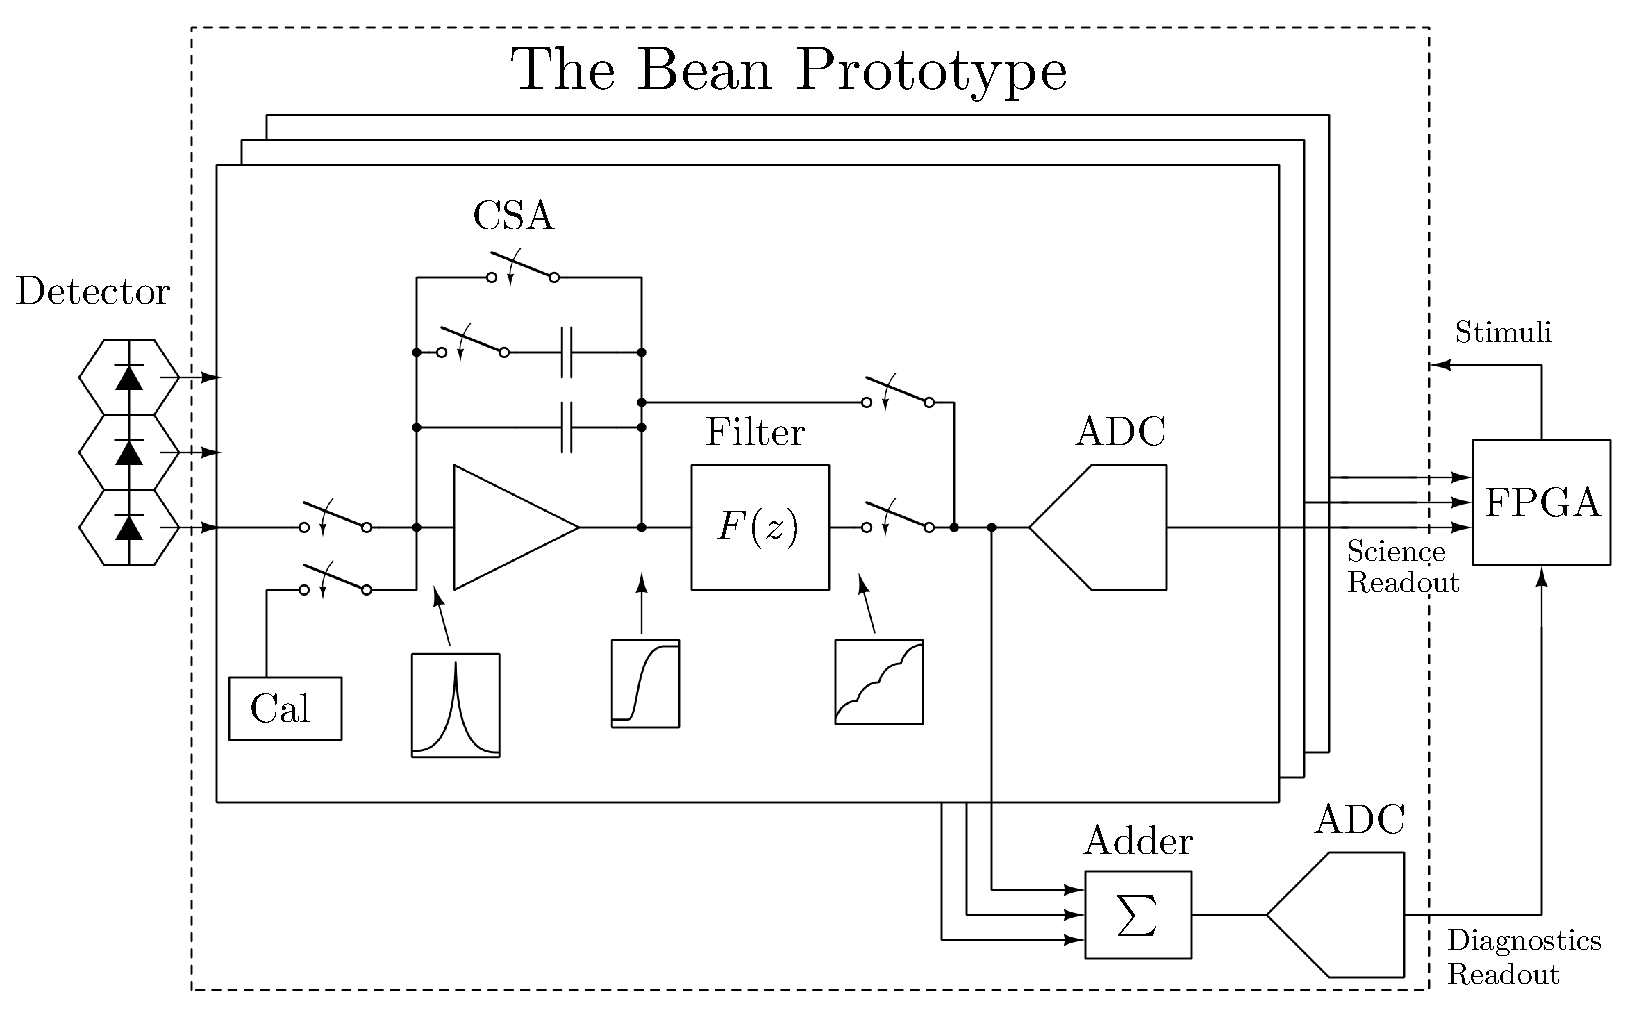
\includegraphics[width=5.3in]{./Figures/thebean_diag.eps}
	\caption{The Bean prototype block diagram.}\label{fig:bean_diag}
\end{figure}

\begin{table}[!t]
	\begin{center}
		\begin{tabular}{|l|l|}\hline
			Input rate & $3.25\,\text{MHz}$ during $0.87\,\text{ms}$, repeated every $200\,\text{ms}$ \\ \hline
			Channels per ASIC & $32$ \\ \hline
			Occupancy & $100\%$ \\ \hline
			Resolution & $10$ bits for individual channels, $8$ bits for fast feedback \\ \hline
			Modes of operation & Standard data taking (SDT), Detector Calibration (DCal) \\ \hline
			Input signals & Up to $40$ pC in SDT, $0.74$ pC in DCal \\ \hline
			Input capacitance & $65$ pF \\ \hline
			Additional feature & Low-latency ($1\,\micro\text{s}$) output \\ \hline
			Additional feature & Internal pulser for electronics calibration \\ \hline
			Radiation tolerance & 1 Mrad ($\text{SiO}_2$) total ionizing dose \\ \hline
			Power consumption & $2.19$ mW per channel \\ \hline
			Total ASIC count & $2836$ \\\hline
		\end{tabular}
		\vspace*{5pt}
		\caption{BeamCal instrumentation ASIC specifications summary.}\label{tab:bean_specs}
	\end{center}
\end{table}

